\chapter{粒子線に対する応答評価試験のための読み出しシステムの開発}
この章では,粒子線に対する応答評価試験のために行なった,外部トリガを処理する機能の追加と,応答評価試験のための準備について述べる.

\section{読み出しシステム概要}
以下に読み出しシステムの概要を示す.主にRD53A搭載のSingle Chip Card(SCC)とFPGAボード,PCを用いて読み出しシステムを構成している.今回は読み出しASICとFPGAボードは,HPC-mDP変換ボードを用いてケーブルにて接続を行い,FPGA内部でASICからのデータ信号の処理を行なった.また,高速通信用インターフェースでPCとFPGAボードを接続し,データ転送を行なった.\\

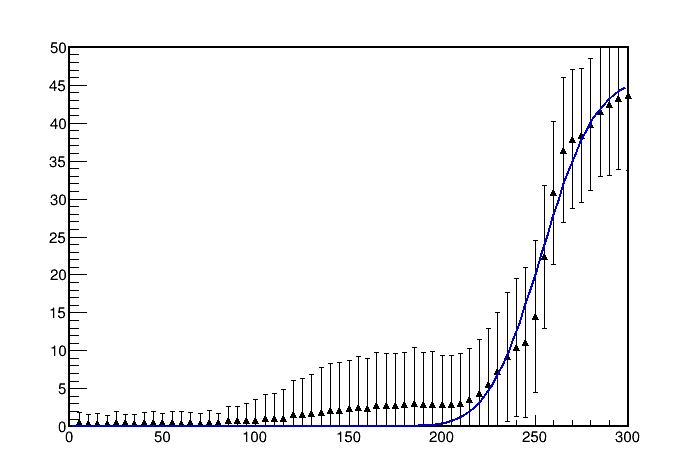
\includegraphics[width=5cm,pagebox=cropbox,clip]{figures/test.pdf}


\subsection{PC}
\subsection{FPGAボード}
\subsection{アダプタカード}
\subsection{RD53A搭載Single Chip Cardモジュール}

\section{外部トリガを処理する機能の追加}
本章では,シリコンピクセルセンサが接続されたRD53Aから出力されるHitOR信号を外部トリガに用いて,機能の動作を検証する.センサ付きRD53Aが搭載された基盤の写真を以下に示す.RD53Aは細い金属ワイヤにより基板上の回路パターンと電気的に接続されている.基板にRD53Aが外部と通信するためのコネクタ,電源供給のためのコネクタ,センサからの信号を外部に出力するためのコネクタ,センサに電圧を印加するためのコネクタが実装されている.RD53Aとのデジタル通信は,コネクタを介して行う.

\subsection{概要}


\section{読み出し準備}
\subsection{閾値チューニング}
\subsection{Latencyチューニング}


